% 能量法解谐振动问题

\pentry{简谐振子\upref{SHO}, 机械能守恒\upref{ECnst}}

由于谐振动系统的总能量是常量,反过来我们可以用机械能守恒定律来导出谐振动的运动方程.仍以弹簧振子为例,在任一时刻,振子作谐振动的总机械能等于势能加上动能,即
\begin{equation}
E=E_{\mathrm k}+E_{\mathrm p}=\frac{1}{2} m v^{2}+\frac{1}{2} k x^{2}
\end{equation}
由于总机械能$E$是常量,不随时间而改变,上式对时间$t$求导得
\begin{equation}
m v \frac{\mathrm{d} v}{\mathrm{d} t}+k x \frac{\mathrm{d} x}{\mathrm{d} t}=0
\end{equation}
由速度和坐标间的关系$v = \dv*{x}{t}$,代入整理后,即得谐振动的运动方程
\begin{equation}
\frac{\mathrm{d}^{2} x}{\mathrm{d} t^{2}}+\frac{k}{m} x=0
\end{equation}

能量法在解简谐运动(广义来说,机械能守恒的)问题中非常有帮助, 下面来看一个例题. 

\begin{example}{考虑弹簧质量的弹簧振子}
当考虑弹簧的质量时,用能量法求解弹簧振子的周期.设弹簧的质量为$m_0$,且小于振动物体的质量$m$,弹簧的劲度系数为$k$,弹簧的原长为$L$.

\begin{figure}[ht]
\centering
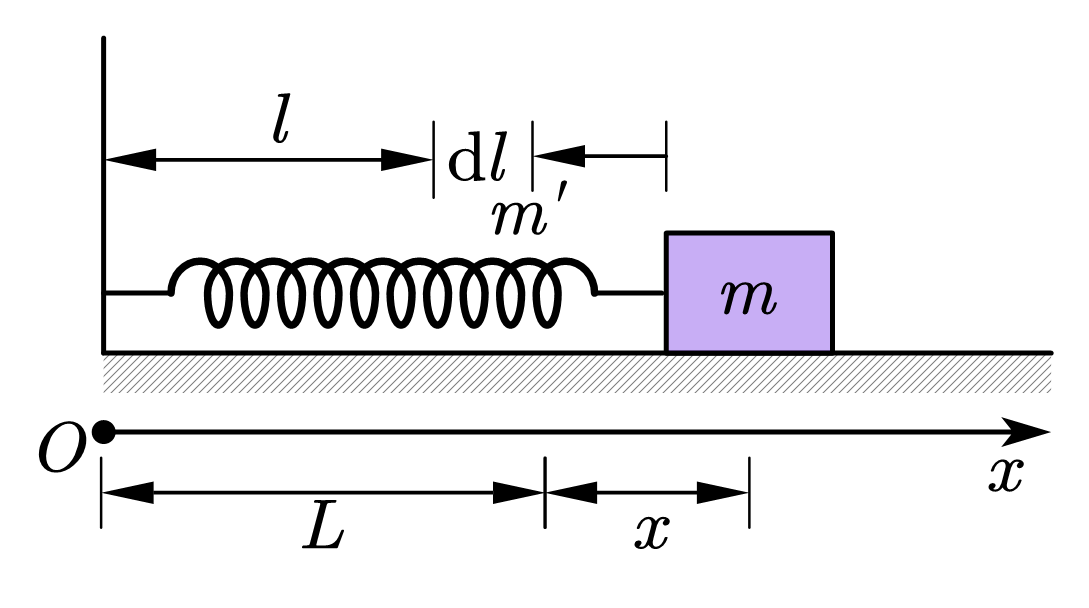
\includegraphics[width=7cm]{./figures/EnerVi_1.png}
\caption{考虑弹簧质量的弹簧振子} \label{EnerVi_fig1}
\end{figure}

在振动过程中任一时刻,设物体的位移为$x $,速度为$v$.如\autoref{EnerVi_fig1}所示.弹簧振动时,可以认为弹簧在振动的任一时刻内,各等长小段的变形相同,弹簧各截面处的位移是线性变化的.在离弹簧固定端距离$l$的地方取一小段微元长度$\mathrm dl$,质量即为$\dfrac{m^\prime}{L}\mathrm{d}l$,位移为$\dfrac{x}{L}l$,因而该段微元长度的速度就等于$\dfrac{v}{L}l$,写出其微元动能的表达式:
\begin{equation}
\mathrm{d} E_{\mathrm{k}}^{\prime}=\frac{1}{2}\left(\frac{m^{\prime}}{L} \mathrm{d} l\right)\left(\frac{l}{L} v\right)^{2}=\frac{m^{\prime} v^{2}}{2 L^{3}} l^{2} \mathrm{d} l
\end{equation}
积分,可得整个弹簧的动能:
\begin{equation}
E_{\mathrm{k}}^{\prime}=\int_{0}^{L} \frac{m^{\prime} v^{2}}{2 L^{3}} l^{2} \mathrm{d} l=\frac{1}{2} \frac{m^{\prime}}{3} v^{2}
\end{equation}
于是,整个弹簧振子系统的总机械能
\begin{equation}
E=\frac{1}{2} k x^{2}+\frac{1}{2} m v^{2}+\frac{1}{2} \frac{m^{\prime}}{3} v^{2}
\end{equation}
由于整个系统没有能量损耗,所以机械能守恒,即
\begin{equation}
\frac{1}{2} k x^{2}+\frac{1}{2} m v^{2}+\frac{1}{2} \frac{m^{\prime}}{3} v^{2}=E=\mathrm{constant}
\end{equation}
将此方程对时间$t $求导,得
\begin{equation}
\left(m+\frac{m^{\prime}}{3}\right) \frac{\mathrm{d}^{2} x}{\mathrm{d} t^{2}}+k x=0
\end{equation}
将其改写成简谐振动的微分方程形式:
\begin{equation}
\frac{\mathrm{d}^{2} x}{\mathrm{d} t^{2}}+\omega^{2} x=0 \qquad \qty(\omega^{2}=\frac{k}{m+m^{\prime} / 3})
\end{equation}
于是可得运动周期:
\begin{equation}
T=\frac{2 \pi}{\omega}=2 \pi \sqrt{\frac{m+m^{\prime} / 3}{k}}
\end{equation}

\end{example}
